\documentclass[11pt]{article}
\usepackage[T1]{fontenc}
\usepackage[utf8]{inputenc}
\usepackage{lmodern}
\usepackage[letterpaper,margin=1in]{geometry}
\usepackage{microtype}
\usepackage{amsmath,amssymb,amsthm,mathtools}
\usepackage{aliascnt}
\usepackage{booktabs,array,tabularx}
\usepackage{graphicx}
\usepackage{algorithm,algpseudocode}
\usepackage{enumitem}
\usepackage{authblk}
\usepackage[backend=biber,style=alphabetic,maxbibnames=99,maxalphanames=4,giveninits=true,doi=true,url=false,isbn=false]{biblatex}
\addbibresource{references.bib}
\usepackage[hidelinks]{hyperref}
\usepackage[nameinlink,noabbrev]{cleveref}
\usepackage{xcolor}
\makeatletter
\providecommand{\theHALG@line}{}
\renewcommand{\theHALG@line}{\thealgorithm.\arabic{ALG@line}}
\makeatother
\hypersetup{pdftitle={Optimal (Parallel) Spooky Pebbling on Binary Trees},pdfauthor={Mingyu Lee, Sanghyun Lee, Kabgyun Jeong},pdfsubject={Space, work, depth, and cumulative occupancy in measurement-assisted pebbling}}

\newtheorem{theorem}{Theorem}[section]
\newaliascnt{lemma}{theorem}
\newtheorem{lemma}[lemma]{Lemma}
\aliascntresetthe{lemma}
\newaliascnt{proposition}{theorem}
\newtheorem{proposition}[proposition]{Proposition}
\aliascntresetthe{proposition}
\newaliascnt{corollary}{theorem}
\newtheorem{corollary}[corollary]{Corollary}
\aliascntresetthe{corollary}
\theoremstyle{definition}
\newaliascnt{definition}{theorem}
\newtheorem{definition}[definition]{Definition}
\aliascntresetthe{definition}
\theoremstyle{remark}
\newaliascnt{remark}{theorem}
\newtheorem{remark}[remark]{Remark}
\aliascntresetthe{remark}
\crefname{lemma}{lemma}{lemmas}
\crefname{proposition}{proposition}{propositions}
\crefname{corollary}{corollary}{corollaries}
\crefname{definition}{definition}{definitions}
\crefname{remark}{remark}{remarks}
\DeclareMathOperator{\pred}{pred}
\DeclareMathOperator{\parv}{par}
\DeclareMathOperator{\topv}{top}
\DeclareMathOperator{\popcount}{popcount}

\newcommand{\Peb}{\mathsf{Pebble}}
\newcommand{\ket}[1]{\lvert#1\rangle}
\newcommand{\Unp}{\mathsf{Unpebble}}
\newcommand{\Ghost}{\mathsf{Ghost}}
\newcommand{\Fast}{\mathsf{SequentialPebble}}
\newcommand{\Release}{\mathsf{Release}}


\newcommand{\Sweep}{\mathsf{ParallelPebble}}
\newcommand{\Clean}{\mathsf{FastClean}}
\newcommand{\Resolve}{\mathsf{Resolve}}
\newcommand{\Contract}{\mathsf{Contract}}
\newcommand{\Forest}{\mathcal F}
\newcommand{\Gstate}{\mathsf G}
\newcommand{\Area}{\mathcal A}
\newcommand{\Wseq}{W_{\mathrm{seq}}}
\newcommand{\Wpar}{W_{\mathrm{par}}}
\newcommand{\Dpar}{D_{\mathrm{par}}}
\newcommand{\cstar}{^{\star}}
\newcommand{\pos}[1]{(#1)_+}
\newcommand{\mingyu}[1]{{\color{magenta}\footnotesize [MINGYU: #1]}} %todo: remove.
\setlist{itemsep=2pt,topsep=4pt}
\setlength{\emergencystretch}{2em}
\allowdisplaybreaks[1]
\floatname{algorithm}{Algorithm}
\algrenewcommand\algorithmicrequire{\textbf{Input:}}
\algrenewcommand\algorithmicensure{\textbf{Output:}}

\title{Optimal (Parallel) Spooky Pebbling on Binary Trees}

\author[1,2]{Mingyu Lee}
\author[2,3]{Sanghyun Lee}
\author[2,4]{Kabgyun Jeong}

\affil[1]{Department of Computer Science and Engineering,
Seoul National University, Seoul 08826, Republic of Korea}

\affil[2]{Team QST,
Seoul National University, Seoul 08826, Republic of Korea}

\affil[3]{Department of Mechanical Engineering,
Kyung Hee University, Yongin 17104, Republic of Korea}

\affil[4]{Institute of Computer Technology, College of Engineering,
Seoul National University, Seoul 08826, Republic of Korea}

\date{}

\begin{document}
\maketitle
\vspace{-1.4em}
\begin{abstract}

Pebble games model computations under a fixed space budget. Spooky pebbling allows quantum memory to be released by measurement, with the resulting phases corrected later. We study two-input computations with binary-tree dependencies and determine their optimal work and parallel depth. For the complete tree $B_h$ with $n=2^h-1$ vertices and every space budget $h+1\le s\le n$, we give an algorithm with asymptotically optimal work $\Theta(nh/\log(s+1))$. We also construct a parallel schedule with optimal depth
\[
 \Theta\!\left(h+\frac ns
 \max\!\left\{\frac{h}{\log(s+1)},\,1+\log^*h\right\}\right).
\]
The work bound resolves the time-optimality question left open by Kornerup, Sadun, and Soloveichik. Our lower bounds hold for every full binary tree. The main idea is to retain the largest balanced boundary allowed by the budget and uncompute the vertices above it before releasing its values. At space $\Theta(n/h)$, the least work of a depth-optimal strategy is $\Theta(n(1+\log^*h))$, whereas the unrestricted work optimum is $\Theta(n)$. Applying our schedule to the RNS point-addition trees in the public implementation of Chevignard, Fouque, and Schrottenloher reduces their evaluation cost by $20.86\%$ for a P-224 instance and $22.66\%$ for a P-256 instance, using the same arithmetic circuits and peak workspace.
\end{abstract}

\section{Introduction}

Consider a quantum out-of-place operation $f$ with $n$ inputs:
\begin{equation}
    \ket{a_1}\cdots\ket{a_n}\ket{0} \longmapsto \ket{a_1}\cdots\ket{a_n}\ket{f(a_1,\ldots,a_n)}.
\end{equation}

This operation must act coherently on superpositions of inputs. When the output of one operation serves as an input to another, the intermediate value must be stored in a quantum register until it is used. Repeatedly combining pairs of values forms a binary tree of computations when each value is used as an input at most once. Such a structure appears when adding elliptic-curve points~\cite{CFS2026}, as we discuss in \cref{sec:cfs-case-study}.

Once an intermediate value is no longer needed, we would like to clear its register to save space. We can do this by reversing the operation that produced the value, but this requires its inputs to remain available. If their registers have already been cleared, those inputs must be computed again. Keeping intermediate values therefore uses more memory, while clearing them early may require more computation.

Pebble games describe this tradeoff between memory and computation~\cite{Bennett1989}. Each vertex represents a value, and its predecessors represent the inputs needed to compute it. A pebble indicates that the value is stored in a register. Placing a pebble corresponds to computing the value, and removing it with its inputs available corresponds to uncomputing it.

Measurement offers another way to release a quantum register. Instead of uncomputing its value, we can measure the register in the Hadamard basis and free it immediately. This reduces the quantum memory in use, but leaves a phase that must be corrected later. Suppose the measured register holds $x$, and let $\ket{\psi_x}$ denote the state of the remaining registers. A measurement outcome $m$ leaves
\begin{equation}
    \sum_x \alpha_x\ket{\psi_x}\ket{x} \longmapsto \sum_x \alpha_x(-1)^{m\cdot x}\ket{\psi_x},
\end{equation}
where $m\cdot x$ is computed modulo two and the measured register has been discarded. The factor $(-1)^{m\cdot x}$ may change the relative phases of the remaining state and therefore affect interference in subsequent quantum operations.

In the pebble game, we represent this pending phase correction by a ghost. Unlike a pebble, a ghost does not occupy a quantum register; the measurement outcome is stored classically. Correcting the phase is called exorcising the ghost. Once the required inputs are available, we can do this by recomputing $x$ and applying $Z$ to each qubit whose corresponding measurement outcome is one. We obtain
\begin{equation}
    \sum_x \alpha_x(-1)^{m\cdot x}\ket{\psi_x}\ket{x} \xrightarrow{\bigotimes_j Z^{m_j}} \sum_x \alpha_x\ket{\psi_x}\ket{x}.
\end{equation}
We can then uncompute $x$ to clear its register without leaving a phase.

This extension of the pebble game, introduced by Gidney, is called spooky pebbling~\cite{Gidney2019}. It allows us to release quantum memory before the inputs needed for uncomputation are available, at the cost of correcting the resulting phases later. A successful strategy must produce the desired output and clear all other pebbles and ghosts. Figure~\ref{fig:binary-pebbling-concept} illustrates a configuration of the spooky pebble game on a binary tree.

\begin{figure}[htbp]
    \centering
    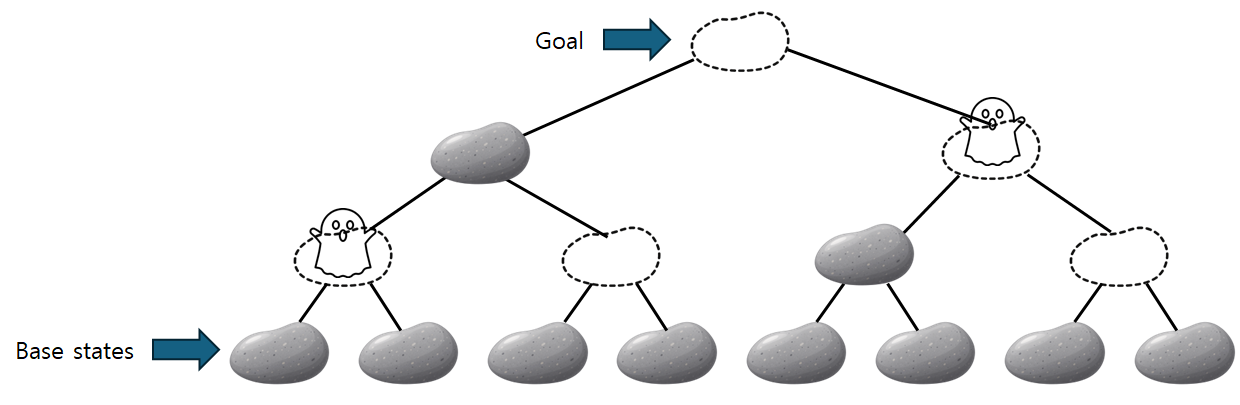
\includegraphics[width=\textwidth]{figs/binary_pebbling_concept.png}
    \caption{Illustration of spooky pebbling on a binary tree. Pebbles represent values stored in quantum registers, and ghosts represent pending phase corrections. Vertices with neither a pebble nor a ghost are empty. The configuration shown here occupies 10 quantum registers. Pebbling or unpebbling an internal vertex requires pebbles on both children. The goal is to leave only the root pebbled, with all other vertices empty.}
    \label{fig:binary-pebbling-concept}
\end{figure}

\subsection{Prior work}

Kornerup, Sadun, and Soloveichik studied sequential spooky pebbling, where one pebble is placed or removed at a time~\cite{KSS2025}. They determined the optimal tradeoff between computation time and memory use for a chain of connected nodes. For a complete binary tree with $h$ vertex levels and $n=2^h-1$ vertices, they constructed a strategy using the minimum $h+1$ pebbles and $O(n\log n)$ steps~\cite[Theorem~5.5]{KSS2025}. Their step count includes placements, uncomputations, and ghosting. The strategy first computes the root, leaving ghosts below it, and then recomputes child values to clear these ghosts. It remained open whether the $O(n\log n)$ bound can be improved, along with the question of a general time--space tradeoff on binary trees~\cite[Section~6]{KSS2025}.

On more general dependency graphs, KSS studied the hardness of minimizing pebble space. Quist and Laarman proved PSPACE-completeness results and developed SAT-based methods to find spooky pebbling strategies with small quantum space, classical space, or execution time~\cite{QL2025}. Our focus is on explicit strategies and matching bounds for binary trees.

Another way to reduce execution time is to perform independent operations in parallel. To formalize this in reversible computing, Blocki, Holman, and Lee introduced parallel reversible pebbling~\cite{BHL2022}. Combining this framework with spooky pebbling, Kahanamoku-Meyer, Ragavan, and Van Kirk (KMRV) introduced parallel spooky pebbling, which also allows registers to be released by measurement~\cite{KMRV2026}. In their model, operations are executed in synchronous rounds: the number of rounds determines the depth, while the total number of computations and uncomputations determines the work. Performing multiple operations in a single round can therefore reduce depth without increasing total work.

KMRV studied this model on a linear chain of $\ell$ vertices, showing that reaching the target and clearing all values requires an optimal $2\ell$ rounds using $O(\log\ell)$ pebbles~\cite{KMRV2026}. They also applied their construction to reduce the depth of arithmetic in Regev's factoring algorithm.

These results leave the tradeoffs on binary trees open. Independent subtrees can be computed in parallel, but both child values must be available to compute or uncompute their parent. Under a fixed space budget, a schedule must decide which subtrees to process concurrently and which values to retain for cleanup. We ask what work and depth are optimal at each space budget, and whether a single strategy can minimize both.

\subsection{Main results}

Let $B_h$ be the complete binary tree of height $h\ge2$, where height counts vertices on a longest root-to-leaf path. Then $B_h$ has $n=2^h-1$ vertices. Write $\Wseq^\star(B_h,s)$ and $\Wpar^\star(B_h,s)$ for the minimum sequential and parallel work with space at most $s$, and $\Dpar^\star(B_h,s)$ for the minimum parallel depth. Also write $\lambda(x)=1+\log^*x$, where $\log^*x$ is the number of iterated binary logarithms needed to reach a value at most one.

\begin{theorem}[Informal, optimal space--work tradeoffs and parallel depth;
see \cref{thm:seq-upper,thm:parallel-upper,thm:universal-work,thm:weighted}]
\label{thm:main}
For every integer $h+1\le s\le n$,
\begin{equation}
    \Wseq^\star(B_h,s)=\Wpar^\star(B_h,s)=\Theta\!\left(\frac{nh}{\log(s+1)}\right).
    \label{eq:main-work}
\end{equation}
The optimal parallel depth is
\begin{equation}
    \Dpar^\star(B_h,s)=\Theta\!\left(h+\frac ns\max\!\left\{\frac{h}{\log(s+1)},\lambda(h)\right\}\right).
    \label{eq:main-depth}
\end{equation}
Work and depth are minimized separately. All implicit constants are absolute and uniform over the entire feasible interval.
\end{theorem}


At the minimum budget $s=h+1$, a single parallel construction attains
\begin{equation}
    W=\Theta\!\left(\frac{n\log n}{\log\log n}\right), \qquad D=\Theta\!\left(\frac n{\log\log n}\right).
    \label{eq:min-space}
\end{equation}
The work bound improves the KSS bound by a factor of $\log\log n$ and resolves their question about time-optimality on complete binary trees. At space $s=\Theta(n)$, linear work and depth $\Theta(h)$ are attainable.

Our lower bounds also allow us to compare different tree shapes. A full binary tree is one in which every internal vertex has exactly two children. For any such tree with $n$ vertices, we prove a work lower bound of $\Omega(n\log n/\log(s+1))$. We also bound how long values must remain in memory. Define cumulative storage as the sum of the space used in each round. Every parallel strategy has cumulative storage $\Omega(n\lambda(n))$, and a strategy with space at most $s$ and depth $D$ has cumulative storage at most $sD$. This gives an additional lower bound on depth. Combining these bounds with our complete-tree constructions gives the following result.

\begin{theorem}[Optimality over tree shapes]
\label{thm:main-shape}
Let $N=2^{h-1}$, and let $\mathcal T_N$ contain all ordered full binary trees with $N$ leaves. At every common budget $h+1\le s\le2N-1$, a complete balanced tree minimizes sequential work, parallel work, and parallel depth up to constant factors over $\mathcal T_N$.
\end{theorem}

For an associative operation, choosing an ordered tree amounts to choosing a parenthesization with the same leaf order. Thus \cref{thm:main-shape} also gives the optimal asymptotic cost over these parenthesizations within the tree model.

Work and depth can require different strategies. At $s=\Theta(n/h)$, the minimum work is $\Theta(n)$, while the minimum depth is $\Theta(h\lambda(h))$. Every strategy attaining this depth performs $\Omega(n\lambda(h))$ work, and our construction attains that work bound. Thus a strategy that minimizes depth in this regime must do asymptotically more work than one that minimizes work alone.

We also apply our cleanup strategy to a fixed point-addition tree in the public implementation of Chevignard, Fouque, and Schrottenloher~\cite{CFS2026}. Their computation uses a residue number system (RNS), evaluating the point-addition formulas modulo several small primes. With the same tree and arithmetic circuits, our strategy reduces per-prime Toffoli/AND-equivalent work by $20.86\%$ for a P-224 instance and $22.66\%$ for the primary P-256 instance, with unchanged peak workspace. These measurements use the costs of the individual circuits rather than unit costs for tree operations. \Cref{sec:cfs-case-study} gives the comparison.

\subsection{Proof overview}


\mingyu{todo: fix this at last}
Our sequential strategy begins by retaining a boundary of subtree values. With those values available, it computes the root and uncomputes the vertices above the boundary before releasing it. This leaves the root pebbled and ghosts only in the smaller subtrees below. To clean each subtree, we again retain boundary values while computing and uncomputing the vertices above them. This clears a block of levels at once. We then release the retained values and repeat on the smaller subtrees. We call this procedure block cleanup.

The space budget determines how many levels can be cleared together. After reserving one pebble for the output, cleanup has budget $b=s-1$. As the remaining subtrees become shorter, the same budget allows more values to be retained and larger blocks to be cleared. This leads to $O(h/\log(s+1))$ cleanup stages, even when the original budget is only $h+1$. The subtrees at any one stage are disjoint, and their total size is $O(n)$. Each stage therefore takes $O(n)$ work, giving the sequential upper bound.

For the work lower bound, we consider the last time each non-output value is removed. This final removal must be an uncomputation: a final measurement would leave a ghost with no later computation to clear it. Its children must therefore be present at that time. Final removals occur from ancestors to descendants. We partition a connected region into smaller connected pieces. When the top vertex of the region is finally removed, the space budget forces many pieces to contain no pebble. Values in those pieces must be recomputed to finish the cleanup below. Repeating this argument at smaller scales gives the required work. The order of final removals ensures that no placement is counted twice.

To reduce depth, we compute independent parts of the tree in parallel. We first show how to compute the root of a height-$r$ subtree with a feasible budget $b$ in $O(r+2^r/b)$ rounds. We use this procedure to prepare the retained values for block cleanup. Initial cleanup stages make the remaining subtrees small enough to process many of them together. We then clear blocks that reduce their heights from $r$ to $O(\log r)$. Each stage takes $O(r+n/b)$ rounds. The heights sum to $O(h)$, but the $n/b$ term is paid at each of $O(\lambda(h))$ stages. This repeated cost produces the iterated-logarithm term in the depth bound.

The matching depth lower bound requires more than counting operations. A value may occupy a register for many rounds while waiting to be used. We again partition the tree into connected pieces and use the order of final removals. Each piece must either keep a pebble for a sufficiently long interval or become empty and later recompute its values. Counting both possibilities across smaller and smaller pieces gives the cumulative-storage lower bound. A stronger form of this argument shows that achieving cumulative storage $O(n\lambda(n))$ requires $\Omega(n\lambda(n))$ work. At space $\Theta(n/h)$, every depth-optimal strategy has cumulative storage at most this order, which proves the separation between minimum work and the work needed for minimum depth.

\section{Pebbling models}
\label{sec:models}

\subsection{Fixed dependency trees}

A rooted full binary tree $T=(V,E)$ has either zero or two children at each vertex. Edges point from children to their parent, so the root $r$ is the unique sink. We write $\pred(v)$ for the children of $v$, and $\parv(v)$ for its parent, when it exists. The height $H(T)$ is the number of vertices on a longest leaf-to-root path. We fix the dependency tree $T$. The complete binary tree $B_h$ has
$2^h-1$ vertices and $2^{h-1}$ leaves.
All logarithms are binary unless stated otherwise.

An internal vertex $v$ computes a function $f_v$ from its two child values using an out-of-place unitary $U_v$ satisfying
\[
U_v\ket{a}\ket{b}\ket{0}=\ket{a}\ket{b}\ket{f_v(a,b)}.
\]
Applying $U_v^\dagger$ uncomputes this value when both child values are available. Leaf values have no dependencies and can be loaded and erased at any time during the computation. The functions $f_v$ may differ between vertices and need not be associative or invertible.

\subsection{Configurations and actions}

A configuration is a pair $(P,G)$ of disjoint subsets of $V$. Vertices in $P$ have pebbles, representing values stored in quantum registers. Vertices in $G$ have ghosts, representing pending phase corrections. All other vertices are empty. We allow three actions:
\[
\begin{array}{lllc}
\text{Action} & \text{Condition} & \text{New configuration} & \text{Work} \\[3pt]
\Peb(v) & v\notin P,\ \pred(v)\subseteq P & (P\cup\{v\},\ G\setminus\{v\}) & 1 \\[3pt]
\Unp(v) & \{v\}\cup\pred(v)\subseteq P & (P\setminus\{v\},\ G) & 1 \\[3pt]
\Ghost(v) & v\in P & (P\setminus\{v\},\ G\cup\{v\}) & 0
\end{array}
\]
When $v\in G$, $\Peb(v)$ also applies the single-qubit phase corrections specified by the stored measurement outcome, clearing the ghost. \mingyu{We should discuss why work doesn't count for ghost. And discuss about kss setting, and why this gives asymptotically same work.}

The initial configuration is $(\varnothing,\varnothing)$, and the goal is $(\{r\},\varnothing)$: retain the root value and clear every other pebble and every ghost.

\subsection{Sequential and parallel execution}

A sequential strategy executes one action at a time. Each $\Peb$, $\Unp$, or $\Ghost$ action is one step.

A parallel strategy executes actions in rounds with two phases, following the execution rule of KMRV~\cite[Section~2.1]{KMRV2026}. In the first phase, $\Peb$ and $\Unp$ actions may run simultaneously if their active sets
\begin{equation}
A_v=\{v\}\cup\pred(v)
\label{eq:active-set}
\end{equation}
are pairwise disjoint. Their preconditions are checked at the beginning of that phase. In the second phase, $\Ghost$ may be applied to any set of currently pebbled vertices. Depth is the number $D$ of rounds.

\subsection{Space and work}
\label{sec:work-counts}

Every pebble occupies one register, including pebbles on leaves. Ghosts occupy no quantum space. Sequential space is the maximum number of pebbles present at any step. For a parallel strategy $\mathcal P$, let $P_t$ be the pebble set after round $t$, and let $P_t^+$ be its pebble set after the first phase, before ghosting. We count every register occupied during a round:
\begin{equation}
U_t=P_{t-1}\cup P_t^+, \qquad s(\mathcal P)=\max_{1\le t\le D}|U_t|, \qquad \Area(\mathcal P)=\sum_{t=1}^D|U_t|.
\label{eq:parallel-resources}
\end{equation}
Here $\Area$ is cumulative storage. External input registers and temporary registers used inside an action are accounted for separately in circuit resource estimates. Classical storage and control are unrestricted.

Work counts function computations and uncomputations: $W = \#\Peb + \#\Unp$. $\Ghost$ releases a register by measurement without evaluating a vertex function, so it contributes no work.

Let $\Pi$ denote the total number of pebble placements ($\#\Peb$) in a complete strategy. Because every placed pebble except the final root must eventually be removed—either by $\Unp$ or by $\Ghost$—the total number of removals is $\Pi - 1$. Consequently, the total action count is $N_{\text{step}} = \Pi + (\Pi - 1) = 2\Pi - 1$, which satisfies
\begin{equation}
    W \le N_{\text{step}} < 2W.
\end{equation}
KSS~\cite{KSS2025} count ghosting as a step, whereas
KMRV~\cite{KMRV2026} count only computations and uncomputations.
Since $W$ and $N_{\mathrm{step}}$ differ by at most a factor of two,
our asymptotic work bounds are unchanged under either convention.


For a dependency tree $T$ and an integer space budget $s$, we denote by $\Wseq^\star(T,s)$ and $\Wpar^\star(T,s)$ the minimum sequential and parallel work, respectively, and by $\Dpar^\star(T,s)$ the minimum parallel depth. If no valid pebbling strategy exists within space $s$, the corresponding value is taken to be $+\infty$.

For complete binary trees $B_h$ of height $h \ge 2$, the space budget has a natural feasible range. Computing the root requires at least $h+1$ pebbles even when measurement-assisted register release is permitted~\cite{Cook1973,KSS2025}. At the other extreme, a budget of $n = 2^h-1$ pebbles allows the entire tree to be held in quantum memory simultaneously. Thus, throughout this paper, our tradeoffs for complete trees focus on the non-trivial feasible interval
\begin{equation}
    h+1 \le s \le 2^h-1.
\end{equation}

Any parallel strategy can be serialized into a sequential one by executing each round's actions in sequence—first $\Unp$, then $\Peb$, and finally $\Ghost$. Because active sets in the first phase are pairwise disjoint, this order preserves preconditions without interference, and all intermediate pebble configurations remain within $U_t$. Conversely, any sequential step can be viewed as a single-action parallel round, which implies
\begin{equation}
    \Wseq^\star(T,s) = \Wpar^\star(T,s).
    \label{eq:serialize}
\end{equation}



\section{Our algorithms}
\label{sec:main-algorithms}

The computation has two parts: compute the root value from the bottom, then clear every other vertex while retaining the root. With space $s=n$, we can hold all vertex values at once. Pebbling the tree bottom-up and unpebbling every non-root vertex top-down uses $n+(n-1)=2n-1$ work. Under a smaller space budget, values must be released before the cleanup that needs them, and recovering those values requires additional work.

The bottom-up \texttt{fast\_pebble} routine of KSS, which we call $\Fast$, computes the root with $O(n)$ work using the minimum feasible $h+1$ pebbles, but leaves ghosts below it. KSS gave an $O(n\log n)$-step strategy to clear these ghosts at the same minimum budget~\cite[Theorem~5.5]{KSS2025}. The additional work comes from reconstructing child values during cleanup. Our strategy retains selected subtree roots while computing a block above them, then uncomputes that block before releasing those values. We develop this block cleanup in \cref{sec:block-cleanup} and analyze its sequential work and parallel depth in the following subsections. \mingyu{We should discuss little bit more about parallel scheduling and work-depth tradeoff.}

\subsection{Bottom-up root calculation}
\label{sec:fast-root}

For a complete subtree $T$ rooted at $v$ with $H(T)=r$, $\Fast(T)$ computes its children recursively, pebbles $v$, and releases the children afterward. An internal child is ghosted because its own children have already been released. This is the bottom-up root-computation routine in the KSS construction~\cite[Theorem~5.5]{KSS2025}. For a pebbled vertex $u$, let $\Release(u)$ mean $\Unp(u)$ if $u$ is a leaf, and $\Ghost(u)$ otherwise.

\begin{algorithm}[H]
\caption{Bottom-up root computation $\Fast(T)$}
\label{alg:fast-root}
\begin{algorithmic}[1]
\Require A complete subtree $T$ rooted at $v$, with every vertex initially empty or ghosted.
\Ensure The root $v$ is pebbled. Every other internal vertex of $T$ is ghosted, and every other leaf is empty.
\If{$T$ consists of one vertex}
 \State $\Peb(v)$; \Return
\EndIf
\State Run $\Fast(T_L)$ and $\Fast(T_R)$ on the child subtrees
\State $\Peb(v)$
\For{each child root $u$ of $v$}
\State $\Release(u)$
\EndFor
\end{algorithmic}
\end{algorithm}

Every vertex is pebbled once, and every leaf other than the root is unpebbled once. Thus $\Fast(T)$ uses $\Theta(2^r)$ work. From an empty tree, this is optimal up to constants for root computation because every vertex must be computed at least once. Space usage peaks at $r+1$ pebbles for $r\ge2$, or one pebble for a leaf. Its root is ready for use, but the internal ghosts still require cleanup.

\subsection{Block cleanup}
\label{sec:block-cleanup}

Our key idea is to clean up the tree in \emph{blocks}. Starting at a subtree's root, extend a block downward as far as the space budget permits. The vertices at its bottom form the boundary $F$. Compute and retain the values at $F$, then pebble the vertices above it upward to the root and unpebble them downward toward $F$. Finally, release $F$ and clean the subtrees rooted there recursively.

For a complete subtree of height $r$, construct a balanced boundary $F$ of $m$ vertices, where $2\le m\le2^{r-1}$, using \cref{alg:boundary}. The vertices of $F$ lie at depths $\lfloor\log m\rfloor$ or $\lceil\log m\rceil$. Compute the values at $F$ with $\Fast$, processing the tallest boundary subtrees first. Pebble the vertices above $F$ from bottom to top, then unpebble them from top to bottom, retaining the root in the output-producing call. Apply $\Release(u)$ to each $u\in F$, and recursively clean the subtree rooted at each such $u$.

Keeping the values at $F$ available during uncomputation avoids repeatedly reconstructing intermediate vertices. Thus sequential block cleanup achieves optimal work $\Theta(nh/\log(s+1))$ under space budget $s$. At the minimum budget $s=h+1$, this is $\Theta(n\log n/\log\log n)$, improving the $O(n\log n)$ bound of KSS~\cite{KSS2025}. At $s=n$, it gives natural optimal work $\Theta(n)$.

\begin{algorithm}[H]
\caption{Constructing a balanced boundary $\mathsf{Boundary}(T,m)$}
\label{alg:boundary}
\begin{algorithmic}[1]
\Require A complete subtree $T$ rooted at $v$ with $H(T)=r$, and a desired boundary size $m$ satisfying $1\le m\le2^{r-1}$.
\Ensure A set $F$ of exactly $m$ vertices forming a balanced boundary of $T$.
\If{$m=1$}
 \State \Return $\{v\}$
\EndIf
\State $F_L\gets\mathsf{Boundary}(T_L,\lceil m/2\rceil)$
\State $F_R\gets\mathsf{Boundary}(T_R,\lfloor m/2\rfloor)$
\State \Return $F_L\cup F_R$
\end{algorithmic}
\end{algorithm}

The space budget determines the largest feasible boundary size $m$, and $\mathsf{Boundary}(T,m)$ gives the corresponding boundary $F$. The vertices above $F$ form the block. $\Contract(T,m,\rho)$ exorcises this block in one pass, retaining the root when $\rho=1$, and returns $F$ for recursive cleanup. \Cref{lem:contract} analyzes the cost of this one-block operation.


\begin{algorithm}[H]
\caption{One-block cleanup $\Contract(T,m,\rho)$}
\label{alg:block-contract}
\begin{algorithmic}[1]
\Require A complete subtree $T$ with $H(T)=r\ge2$. Its leaves are empty, and each internal vertex is either empty or ghosted.
\Require A boundary size $m$ satisfying $2\le m\le2^{r-1}$, and a flag $\rho\in\{0,1\}$ indicating whether to retain the root of $T$.
\Ensure The boundary $F$ is returned, and all ghosts in the block above $F$ are exorcised. Within $T$, only its root remains pebbled when $\rho=1$; no pebbles remain there when $\rho=0$. Any remaining ghosts lie in the subtrees rooted at $F$.
\State $F\gets\mathsf{Boundary}(T,m)$
\State Compute and retain $F$ using $\Fast$, tallest subtrees first
\State Pebble the vertices above $F$ bottom-up
\State Unpebble them top-down, except the root when $\rho=1$
\State Apply $\Release(u)$ to each $u\in F$
\State \Return $F$
\end{algorithmic}
\end{algorithm}



\begin{lemma}[Cost of one-block cleanup]
\label{lem:contract}
For $r\ge2$ and $2\le m\le2^{r-1}$, $\Contract(T,m,0)$ has peak space and work
\begin{align}
 S(r,m)&=\max\{2m-1,\ r+m-\lceil\log m\rceil\}, \label{eq:boundary-space}\\
 K(r,m)&=3\cdot2^{r-1}+m-2. \label{eq:block-work}
\end{align}

It leaves no pebbles and confines all ghosts to the boundary subtrees. $\Contract(T,m,1)$ retains the root, reducing the work by one without changing the peak space.
\end{lemma}

\begin{proof}
The boundary $F$ has $m$ vertices, and the block above it has $m-1$ vertices. At the end of the upward pebbling pass, all $2m-1$ vertices are pebbled.

The other possible space peak occurs while preparing $F$. Put $q=r-\lceil\log m\rceil$. Its boundary subtrees have height $q$ or $q+1$, and we compute the taller ones first. A balanced boundary has at least two height-$q$ subtrees. Thus a taller computation starts with at most $m-3$ roots retained and uses at most $m+q-1$ pebbles. The final height-$q$ computation starts with $m-1$ roots retained and uses $m+q$ pebbles if $q\ge2$, or $m$ if $q=1$. Together with the top-block peak, this gives \cref{eq:boundary-space}.

For work, each of the $2^r-1$ vertices is pebbled once. The $2^{r-1}$ leaves are unpebbled once, as are the $m-1$ vertices above $F$; all other removals are ghostings. Since work counts only pebbling and unpebbling,
\[
 K(r,m)=(2^r-1)+2^{r-1}+(m-1).
\]
The top vertices are unpebbled while their children are present. Keeping the output root skips one unpebbling.
\end{proof}

For an equal-depth boundary with $b$ registers allocated to the current block, the space conditions become
\begin{equation}
 m+q\le b,\qquad 2m-1\le b,\qquad m=2^k,\quad q=r-k.
 \label{eq:feasible-cut}
\end{equation}

\subsection{Sequential work analysis}
\label{sec:sequential}

We now analyze how block cleanup reduces total work. \Cref{sec:lower-bounds} shows that the resulting bound is asymptotically optimal.

At a height-$r$ cleanup call with budget $b$, choose the largest $m$ satisfying $S(r,m)\le b$. Since $S(r,m)$ is nondecreasing in $m$, binary search finds this value. Within the balanced recursive scheme using $\Fast$, making this choice at every call minimizes total work, including cleanup of the boundary subtrees; see \cref{prop:greedy-boundary}.

\mingyu{Starts from here!}

The procedure $\Clean$ combines one-block cleanup with recursive calls on the boundary subtrees. Its initial call $\Clean(B_h,s,1)$ retains the output root; every recursive call uses $\rho=0$ and clears its subtree completely.

\begin{algorithm}[H]
\caption{Complete-tree block cleanup $\Clean(T,b,\rho)$}
\label{alg:seq-clean}
\begin{algorithmic}[1]
\Require A complete subtree $T$ with $H(T)=r$.
\Require A space budget $b\ge r+1$ for $r\ge2$ ($b\ge1$ for a leaf), a flag indicating whether to retain the root of $T$.
\Ensure Exorcise $T$ and clear all its pebbles, retaining the root when $\rho=1$.
\If{$r=1$}
 \State Place the root if $\rho=1$; \Return
\EndIf
\State Choose the largest $2\le m\le2^{r-1}$ with $S(r,m)\le b$
\State $F\gets\Contract(T,m,\rho)$
\State For each $v\in F$, run $\Clean(T_v,b-\rho,0)$ sequentially
\end{algorithmic}
\end{algorithm}

Each recursive call starts with internal ghosts and empty leaves. Since each boundary subtree has height at most $r-1$, the remaining budget $b-\rho$ is feasible. For analysis, we write $b=s-1$ for the budget available below the output.

Each block costs constant work per leaf, so we bound the number of blocks containing any given leaf. A balanced boundary may span two adjacent depths, so we introduce $k_b(r)$, the largest feasible equal-depth cut depth, to lower-bound the height decrease along every branch. The chosen boundary contains at least $2^{k_b(r)}$ vertices, so every recursive branch loses at least $k_b(r)$ levels.

\begin{lemma}[Number of cleanup stages]
\label{lem:slack}
Suppose $b\ge h$ and $r_0\le h-1$. At each height $r$ with $2^r-1>b$, let $k_b(r)$ be the largest cut depth satisfying \cref{eq:feasible-cut}. Any sequence that decreases $r$ by at least $k_b(r)$ at each stage reaches $2^r-1\le b$ in $O(1+h/\log(b+1))$ stages.
\end{lemma}
\begin{proof}
Put $a=b-r\ge1$. This gap increases as the remaining height decreases. The two cut conditions in \cref{eq:feasible-cut} become
\[
2^k-k\le a,\qquad 2^{k+1}-1\le b.
\]
Choose $k\ge1$ maximally with $2^k\le\min\{a+1,(b+1)/2\}$. Since the subtree does not fit in $b$, we have $k<r$, and both cut conditions hold. Hence, for an absolute constant $c>0$,
\[
 k_b(r)\ge c\min\{\log(a+1),\log(b+1)\}.
\]
Each cut reduces $r$, and thus increases $a$, by at least $k_b(r)$.

Once $a\ge\sqrt b$, every nonterminal cut removes $\Omega(\log(b+1))$ levels. The remaining height is at most $h$, so there are $O(h/\log(b+1))$ such cuts. If $b\ge2h$, the initial gap already exceeds $\sqrt b$. Otherwise $h\le b<2h$; because every cut removes at least one level, at most $\lceil\sqrt b\rceil=O(h/\log(b+1))$ cuts are needed to reach this threshold. This proves the claimed bound.
\end{proof}

\begin{theorem}[Work analysis of $\Clean$ ]
\label{thm:seq-upper}
For $n=2^h-1$ and $h+1\le s\le n$, \cref{alg:seq-clean} uses at most $s$ pebbles and work $W=O(nh/\log(s+1))$.
\end{theorem}
\begin{proof}

After the first call to $\Contract$, which costs $O(n)$ work, the remaining task is to clean boundary subtrees of height at most $h-1$ using budget $b=s-1$. For any subsequent height-$r$ subtree with $2^r-1>b$, the largest feasible balanced boundary contains at least $2^{k_b(r)}$ vertices, so every recursive branch loses at least $k_b(r)$ levels.

We count the remaining work by distributing each $\Contract$ call's cost equally among the leaves of its subtree:
\begin{itemize}
    \item By \cref{eq:block-work}, each leaf is charged $O(1)$ work per call.
    \item By \cref{lem:slack}, each leaf participates in $O(1+h/\log(b+1))$ calls, including at most one final call once its remaining subtree fits within $b$.
    \item Thus each leaf is charged $O(1+h/\log(b+1))$ work in total.
\end{itemize}
There are $(n+1)/2$ leaves. Adding the first call's work gives
\[
W=O(n)+O\!\left(n\left(1+\frac{h}{\log(b+1)}\right)\right)
 =O\!\left(\frac{nh}{\log(s+1)}\right),
\]
where $b+1=s$, $\log s=\Theta(\log(s+1))$, and $\log(s+1)\le h$ because $s\le n=2^h-1$.

Also, by \cref{eq:boundary-space}, the space bound holds throughout the process.

\end{proof}

\subsection{Parallel depth upper bound}
\label{sec:parallel-upper}

We now derive a depth upper bound for parallel spooky pebbling at every feasible space budget. The schedule parallelizes both boundary preparation and the cleanup of independent subtrees. Once block cleanup has reduced the subtrees sufficiently, we allocate the space among several jobs and process them in parallel batches. Equal-depth boundaries give these jobs a common height, so they can follow the same schedule.
At the minimum budget $s=h+1$, our schedule achieves depth $O(n/\log\log n)$. The matching lower bound in \cref{eq:universal-depth} establishes asymptotic optimality.

For the initial root computation and boundary preparation, we use $\Sweep(q,b)$, a parallel counterpart of $\Fast$ that computes and retains the root of a height-$q$ subtree using at most $b$ registers. It overlaps independent computations and ghosts every non-root value after use, including leaves. These ghosts are removed during the subsequent cleanup.

\begin{lemma}[Parallel root computation]
\label{lem:sweep}
For a complete subtree of height $q$ and space budget $b\ge q+1$, a procedure $\Sweep(q,b)$ computes and retains its root in depth
\begin{equation}
O\!\left(q+\frac{2^q}{b}\right).
\label{eq:sweep}
\end{equation}
It starts with no pebbles and any set of ghosts, pebbles every vertex once, and ghosts every non-root vertex after its parent uses it.
\end{lemma}

The bound combines the dependency height with the cost of processing the tree under budget $b$. \Cref{app:sweep} constructs the schedule even near the minimum $q+1$. A single leaf needs one round and one register.

To clear one block, choose a cut of depth $k$, with $m=2^k$ boundary subtrees of height $q=r-k$. The conditions $m+q\le b$ and $2m-1\le b$ in \cref{eq:feasible-cut} cover the two space peaks: preparing the boundary while retaining completed roots, and storing the boundary together with the vertices above it. We prepare the boundary with $\Sweep$, then compute and uncompute the top block one level per round. Vertices on a common level have disjoint active sets.

\begin{lemma}[Parallel block cleanup]
\label{cor:parallel-contraction}
For every cut satisfying \cref{eq:feasible-cut}, a height-$r$ subtree with no pebbles and arbitrary ghosts can be reduced to its $m$ boundary subtrees with $O(2^r)$ work, space at most $b$, and depth
\begin{equation}
O\!\left(r+\frac{2^r}{b}\right).
\label{eq:parallel-contraction}
\end{equation}
The block finishes with no pebbles, and all remaining ghosts lie in the boundary subtrees.
\end{lemma}
\begin{proof}
Use $\Sweep$ to prepare and retain the boundary roots. The batching construction in \cref{lem:frontier} reserves space for roots already completed and uses the remaining space for active computations. It takes $O(q+m2^q/b)$ rounds and $O(m2^q)$ work.

With the boundary present, the $k$ levels above it take $k$ rounds to pebble and $k$ rounds to unpebble, using $2(m-1)$ work. Apply $\Release$ to the boundary roots in one further round, adding at most $m$ work. Both phases fit by \cref{eq:feasible-cut}, and substituting $q+k=r$ and $m2^q=2^r$ gives the stated bounds.
\end{proof}

To process smaller subtrees together, give each height-$r$ job enough space for one block to take $O(r)$ rounds. By \cref{eq:parallel-contraction}, a local budget of order $2^r/r$ suffices. We use
\begin{equation}
p(r)=\min\left\{2^r-1,\left\lceil\frac{16\cdot2^r}{r}\right\rceil\right\}.
\label{eq:resolver-space}
\end{equation}
The budget $p(r)=\Theta(2^r/r)$ is nondecreasing. It allows up to $\lfloor b/p(r)\rfloor$ jobs to run together, each reducing its height to $O(\log r)$. The routine $\Resolve$ processes all jobs of a height in batches, then repeats on the smaller subtrees. These repeated height reductions produce the iterated logarithm in its cost.

\begin{lemma}[Parallel cleanup of a forest]
\label{lem:resolver}
If $b\ge p(r)$, a procedure $\Resolve(A,r,b)$ clears $A$ disjoint height-$r$ subtrees containing ghosts but no pebbles, with space at most $b$, work $O(A2^r\lambda(r))$, and depth
\begin{equation}
O\!\left(r+\frac{A2^r}{b}\lambda(r)\right).
\label{eq:forest-cleanup}
\end{equation}
\end{lemma}
\begin{proof}
Let $a$ and $t$ be the number and height of the subtrees at the current stage. Put $M=a2^t$, twice the number of their leaves. Initially $M=A2^r$. A block replaces one height-$t$ subtree by $m$ height-$q$ subtrees with $m2^q=2^t$, so $M$ is unchanged between stages.

For $t>16$, choose
\begin{equation}
q=\lceil\log t\rceil+2, \qquad m=2^{t-q}.
\label{eq:resolver-cut}
\end{equation}
Then $4t\le2^q<8t$, so $m\le2^t/(4t)$ and $q\le t/2\le2^t/(4t)$. Both cut conditions hold with the local budget $p(t)$. By \cref{cor:parallel-contraction}, one job takes $O(t)$ rounds and $O(2^t)$ work.

Run at most $\lfloor b/p(t)\rfloor$ disjoint jobs concurrently; their assigned budgets sum to at most $b$. Monotonicity of $p$ ensures that at least one job fits at every stage. The $O(1+ap(t)/b)$ batches take altogether
\begin{equation}
O\!\left(\left(1+\frac{ap(t)}b\right)t\right)=O(t+M/b)
\label{eq:forest-phase}
\end{equation}
rounds and $O(M)$ work. Each batch leaves no pebbles, so its registers can be reused. After processing all $a$ jobs, replace $(a,t)$ by $(am,q)$. At $t\le16$, each subtree fits within $p(t)=2^t-1$: pebble it bottom-up and unpebble it top-down using the same batches. This also clears any leaf ghosts.

For $t>16$, the height update $f(t)=\lceil\log t\rceil+2$ satisfies $f(t)\le t/2$. Thus the heights over all stages sum to $O(r)$. Moreover, $f(f(t))\le\log t$ for $t\ge256$, so there are $O(\lambda(r))$ stages. Summing \cref{eq:forest-phase} gives $O(r+M\lambda(r)/b)$ rounds. Each stage costs $O(M)$ work, giving the work bound.
\end{proof}

The complete schedule uses the full cleanup budget while $p(r)>b$ and switches to $\Resolve$ once $p(r)\le b$, with $b=s-1$ after reserving the output register.

\begin{algorithm}[H]
\caption{Parallel block cleanup on complete trees}
\label{alg:parallel-tree}
\begin{algorithmic}[1]
\Require An initially empty complete binary tree $B_h$ of height $h\ge2$, and a total space budget $s$ satisfying $h+1\le s\le2^h-1$.
\Ensure All ghosts in $B_h$ are exorcised, leaving its root pebbled and every other vertex empty.
\State Run $\Sweep(h,s)$ and retain the root; set $b\gets s-1$
\State Start with the two child subtrees: $(A,r)\gets(2,h-1)$
\While{$p(r)>b$}
 \State Choose the largest $1\le k<r$ satisfying \cref{eq:feasible-cut}
 \State Clear that block in each subtree using \cref{cor:parallel-contraction}, one subtree at a time
 \State Replace the pending forest by its boundary subtrees: $(A,r)\gets(A2^k,r-k)$
\EndWhile
\State Run $\Resolve(A,r,b)$ on the pending forest
\end{algorithmic}
\end{algorithm}

\begin{theorem}[Parallel upper bound]
\label{thm:parallel-upper}
For $n=2^h-1$ and $h+1\le s\le n$, \cref{alg:parallel-tree} uses at most $s$ pebbles and achieves
\begin{align}
D&=O\!\left(h+\frac{nh}{s\log(s+1)}+\frac{n\lambda(h)}s\right), \label{eq:depth-upper}\\
W&=O\!\left(n\left(\frac h{\log(s+1)}+\lambda(h)\right)\right). \label{eq:depth-schedule-work}
\end{align}
\end{theorem}
\begin{proof}
Throughout cleanup, the number $A$ and height $r$ of the pending subtrees satisfy $A2^r=n+1$. In the first part, $p(r)>b$ implies both $2^r-1>b$ and $b<16\cdot2^r/r$. Hence the depth of one block, $O(r+2^r/b)$, is $O(2^r/b)$. Processing all $A$ blocks of that height takes
\[
A\,O(r+2^r/b)=O(n/b)
\]
rounds and $O(n)$ work. The largest feasible cut is used at each stage, so \cref{lem:slack} bounds their number by $O(h/\log(b+1))$.

At the transition, \cref{lem:resolver} adds $O(h+n\lambda(h)/b)$ rounds and $O(n\lambda(h))$ work. The initial root computation takes $O(h+n/s)$ rounds and $n$ work. Adding these costs and using $b=\Theta(s)$ proves the bounds. The retained root occupies one register, and every cleanup stage fits within the other $b$ registers.
\end{proof}

The $nh/\log(s+1)$ work term comes from the large-subtree stages; the $n\lambda(h)$ term comes from repeated batched cleanup. Dividing space among jobs lets more of them run concurrently but can require more cleanup stages. \Cref{sec:separation} identifies budgets where additional work is necessary for optimal depth.

When $s=\Theta(n)$, a direct block schedule attains both $O(n)$ work and $O(h)$ depth. Choose a feasible equal-depth boundary with $\Theta(s)$ roots, so its subtrees have constant height. Prepare the boundary with $\Sweep$, compute and uncompute the top block while retaining the output, and fully clean the remaining subtrees in parallel batches.

\section{Lower bounds}
\label{sec:lower-bounds}

Every vertex must be pebbled at least once, giving $\Pi\ge n$. Stronger bounds follow from cleanup: required child values must either remain available or be reconstructed. We charge this storage and recomputation to intervals determined by final uncomputations, ensuring that different parts of the argument do not count the same cost twice.

\subsection{Regeneration intervals}

A non-output vertex's final removal must be an $\Unp$ action: a final $\Ghost$ would leave a ghost with no later placement to clear it. Write $\tau(v)$ for the step of this final removal in a sequential strategy, or its round in a parallel strategy. A parent must have both children pebbled when it is uncomputed, so their final uncomputations occur later. In parallel execution, overlapping active sets also prohibit these actions from sharing a round. Hence, for every non-output $v$ and descendant $u$,
\begin{equation}
 \tau(u)-\tau(v)\ge\operatorname{dist}(v,u).
 \label{eq:final-removal}
\end{equation}

For a connected region $C$, let $\topv(C)$ be its vertex nearest the root. We partition $C$ into pieces of comparable size, then examine which contain pebbles after $\topv(C)$ is finally removed.

\begin{lemma}[Partitioning a connected region]
\label{lem:partition}
A tree of maximum degree at most three and size $m>a\ge1$ can be partitioned into connected pieces with $a/4<|Q|\le a$.
\end{lemma}
\begin{proof}
For a tree of size $m\ge4$, a centroid's largest adjacent component has size between $(m-1)/3\ge m/4$ and $m/2$. Cutting that edge leaves two parts of sizes between $m/4$ and $3m/4$; sizes two and three are immediate. Repeatedly split parts larger than $a$. Each final part has size at most $a$ and was split from a part larger than $a$, so its size exceeds $a/4$.
\end{proof}

For a piece $Q$, its top must be pebbled when its parent $p$ is finally removed. We charge for providing that value between the final removals of $\topv(C)$ and $p$. A time boundary below means the configuration after a step or complete round. The relevant distinction is whether $Q$ contains a pebble, regardless of ghosts.

\begin{lemma}[Regeneration charges]
\label{lem:charging}
Fix a successful strategy and a connected region that excludes the output. Recursively partition it into connected pieces. For a piece $Q$ of a region $C$, suppose $p=\parv(\topv(Q))$ lies strictly below $\topv(C)$, and define
\begin{equation}
 I(C,Q)=\{\tau(\topv(C))+1,\ldots,\tau(p)\}.
 \label{eq:charge-interval}
\end{equation}
If $Q$ contains no pebbles at some boundary from $\tau(\topv(C))$ through $\tau(p)-1$, then at least $|Q|$ placements occur in $Q\times I(C,Q)$. Ghosts may be present at that boundary. Otherwise, in a parallel execution, $Q\times I(C,Q)$ contributes at least $|I(C,Q)|$ occupied vertex--round pairs to $\Area$. These sets are pairwise disjoint over all such region--piece pairs.
\end{lemma}
\begin{proof}
To finally unpebble $p$, the strategy needs a pebble on $\topv(Q)$. If $Q$ previously contained no pebbles, producing this value requires every vertex in the connected piece $Q$ to be pebbled again. These placements occur after that boundary and before the final removal of $p$, so they lie in $Q\times I(C,Q)$. If instead $Q$ contains a pebble at every relevant boundary $t$, that pebble belongs to $U_{t+1}$ and contributes one occupied vertex--round pair.

For disjoint pieces, the charged vertices are disjoint. For nested pieces, consider a charge inside $Q$ from the outer partition. Its interval ends at $\tau(\parv(\topv(Q)))$, strictly before $\tau(\topv(Q))$ by \cref{eq:final-removal}. Any charge from a region contained in $Q$ starts after $\tau(\topv(Q))$. Thus nested charges use disjoint time intervals, and no placement or occupied vertex--round pair is counted twice.
\end{proof}

\subsection{Work}

At most $s$ pieces can contain pebbles at once. We choose piece sizes so that these occupied pieces cover only a fraction of their region. The rest must be reconstructed, yielding repeated work as we partition further.

\begin{theorem}[Work lower bound]
\label{thm:universal-work}
Every sequential strategy on a full binary tree with $n$ vertices and space at most $s$ has
\begin{equation}
\Pi=\Omega\!\left(\frac{n\log n}{\log(s+1)}\right).
\label{eq:universal-work}
\end{equation}
\end{theorem}
\begin{proof}
If $\log n/\log(s+1)$ is bounded, $\Pi\ge n$ suffices. Otherwise start with the larger child subtree of the output, whose size is at least $(n-1)/2$. This region excludes the output, so every one of its vertices has a final uncomputation.

For a connected region $C$ of size $m>8(s+1)$, apply \cref{lem:partition} with $a=\lfloor m/(4(s+1))\rfloor$. Each resulting piece satisfies
\begin{equation}
 \frac{m}{32(s+1)}<|Q|\le a.
 \label{eq:work-partition}
\end{equation}
Immediately after $\topv(C)$ is finally removed, discard from the count its own piece and the at most $s$ pieces containing pebbles. Their total size is at most $(s+1)a\le m/4$. Thus pieces containing no pebbles have total size at least $3m/4$.

For any such piece $Q$, the parent of $\topv(Q)$ lies strictly below $\topv(C)$. Indeed, if $\topv(Q)$ were an immediate child of $\topv(C)$, it would still be pebbled immediately after that sequential uncomputation. By \cref{lem:charging}, these pieces require at least $3m/4$ later placements within their charge intervals.

Repeat inside every piece, including the pieces discarded from the count at this stage. The charges remain disjoint by \cref{lem:charging}. By \cref{eq:work-partition}, a piece's size decreases by at most a factor $32(s+1)$ at each partition. Consequently each vertex of the initial region belongs to $\Omega(\log n/\log(s+1))$ nonterminal regions. At each partition depth the sum of the region sizes counts their vertices, so summing the regional charges proves the bound.
\end{proof}

The serialization in \cref{sec:work-counts} preserves placements and space. Therefore the same placement lower bound holds for parallel strategies. Since $W\ge\Pi$, it is also a work lower bound in either execution model.

\subsection{Storage and depth}
\label{sec:area}

Dependencies require at least $H(T)$ rounds to reach the root. The placement count and cumulative storage give further constraints: each placement contributes to the occupied registers of its round, and each round occupies at most $s$ registers. Thus
\begin{equation}
\Pi\le\Area\le sD.
\label{eq:capacity}
\end{equation}
The work lower bound already gives $D\ge\Pi/s$. We obtain another bound by charging for values that must remain stored over long intervals.

Set $L=\lambda(n)$. In a region of size $m$, we use pieces of size $\Theta(\log m/L)$. A constant fraction of the region lies in pieces whose parents are $\Omega(\log m)$ levels below the region's top. By \cref{eq:final-removal}, their charge intervals have length at least $L$ times the piece size, with the constants chosen as in \cref{app:storage}. Each piece must either be reconstructed or retain a pebble at every relevant time boundary, contributing at least its size to $\Pi+\Area/L$. The logarithmic reduction in piece size permits $\Omega(L)$ chargeable scales; the appendix proves the required depth of this partition recursion.

\begin{theorem}[Storage and recomputation]
\label{thm:weighted}
There is an absolute constant $c>0$ such that every parallel strategy on a full binary tree with $n$ vertices satisfies
\begin{equation}
\Pi+\frac{\Area}{L}\ge cnL, \qquad L=\lambda(n)=1+\log^*n.
\label{eq:weighted}
\end{equation}
\end{theorem}

Because $\Pi\le\Area$, the theorem implies $\Area=\Omega(n\lambda(n))$, and hence $D=\Omega(n\lambda(n)/s)$. Combining this with the dependency bound and \cref{thm:universal-work} gives
\begin{equation}
D=\Omega\!\left(H(T)+\frac ns\max\!\left\{\frac{\log n}{\log(s+1)},\lambda(n)\right\}\right).
\label{eq:universal-depth}
\end{equation}
For a complete tree, $\log n=\Theta(h)$ and $\lambda(n)=\Theta(\lambda(h))$. These work and depth lower bounds match \cref{thm:seq-upper,thm:parallel-upper}, proving \cref{thm:main}. Keeping the two terms separate in \cref{eq:weighted} will also let us bound the work of a depth-optimal strategy.

\section{Work, depth, and tree shape}

\subsection{Work needed for optimal depth}
\label{sec:separation}

We have determined the minimum work and the minimum depth at each space budget. They need not be attained by the same strategy. At $s=\Theta(n/h)$, \cref{eq:main-work,eq:main-depth} give
\[
\Wpar^\star(B_h,s)=\Theta(n), \qquad \Dpar^\star(B_h,s)=\Theta(h\lambda(h)).
\]
A strategy with this depth cannot afford enough cumulative storage to avoid the recomputations charged by \cref{eq:weighted}. Its work must therefore exceed the linear optimum.

\begin{theorem}[Work at optimal depth]
\label{thm:separation}
For complete trees and budgets $s=\Theta(n/h)$, every family of strategies respecting these budgets and having depth $O(h\lambda(h))$ has work $\Omega(n\lambda(h))$. This order is attained by \cref{alg:parallel-tree}.
\end{theorem}
\begin{proof}
The space and depth bounds give $\Area\le sD=O(n\lambda(n))$. Set $L=\lambda(n)$. Then $\Area/L=O(n)$, whereas the right-hand side of \cref{eq:weighted} is $cnL$. For sufficiently large $L$, the difference must be supplied by $\Pi$, yielding $\Pi=\Omega(nL)$. Bounded $L$ is covered by $\Pi\ge n$. Since $W\ge\Pi$ and $\lambda(n)=\Theta(\lambda(h))$, this proves the required work bound.

For the construction, $s=\Theta(n/h)$ gives $\log(s+1)=\Theta(h)$. Substitution into \cref{thm:parallel-upper} yields work $O(n\lambda(h))$ and depth $O(h\lambda(h))$, attaining both bounds in the statement.
\end{proof}

For budgets with $h/\log(s+1)=\Omega(\lambda(h))$, the additional $n\lambda(h)$ term in the parallel construction is absorbed by $nh/\log(s+1)$. Its work then matches \cref{eq:main-work}, while its depth remains optimal. This includes the minimum budget $s=h+1$.

\subsection{Choosing the evaluation tree}
\label{sec:tree-shape}

For associative operations, choosing the evaluation tree amounts to parenthesizing the same ordered inputs. The universal bounds let us compare these choices at a common space budget.

\begin{proof}[Proof of \cref{thm:main-shape}]
Every ordered full binary tree with $N=2^{h-1}$ leaves has $n=2N-1$ vertices and height at least $1+\log N=h$. Apply \cref{thm:universal-work,eq:universal-depth}. At every budget in the statement, the complete tree is feasible and attains both lower-bound orders by \cref{thm:main}.
\end{proof}

\section{Application to RNS point-addition trees}
\label{sec:cfs-case-study}

Chevignard, Fouque, and Schrottenloher (CFS) evaluate binary trees of elliptic-curve point additions in a residue number system~\cite{CFS2026}. Leaves perform window lookups; internal vertices evaluate projective point-addition formulas modulo an RNS prime. We apply block cleanup to these fixed trees using the costs of the public arithmetic circuits. Both schedules use the same input order, arithmetic kernels, and final output operation.

Work is the Toffoli/AND-equivalent circuit count, and space includes stored values and active-circuit scratch. For a ghost-only block, prepare the boundary and compute the vertices above it except the top. With the top's children available, clear its ghost using the public direct phase-correction circuit in place of its pebble--unpebble pair. Then uncompute the intermediate vertices and release the boundary. Circuit costs determine which boundaries fit and which save work.

Fix the workspace cap, and let $C(v)$ be the minimum cost within this recursive block scheme for clearing the subtree rooted at $v$, starting with internal ghosts and empty leaves. If $c(v,F)$ includes one block's boundary preparation, top cleanup, and boundary release, then
\begin{equation}
 C(v)=\min_{F\ \mathrm{feasible}}\left(c(v,F)+\sum_{u\in F}C(u)\right),
 \qquad C(v)=0\ \text{at a leaf}.
 \label{eq:cfs-cut-work}
\end{equation}
The leaf base case is zero because the block using a leaf already pays for preparing and releasing it. Boundary computations are ordered by decreasing individual peak space, and feasibility includes the scratch of each active circuit. The initial output block starts from an empty tree and uses the published root-update circuit; we charge its cost separately.

\Cref{tab:cfs-application} gives the per-prime work for the entire tree subroutine. The P-224 and P-256 trees have 17 and 19 leaves. In both cases the root circuit leaves room for only its two children, fixing the initial cut. The improvement comes from subsequent cleanup blocks, where the workspace allows up to four boundary values. We enumerate all mixed-depth cuts within this recursive scheme.

\begin{table}[H]
\centering
\small
\setlength{\tabcolsep}{3.2pt}
\renewcommand{\arraystretch}{1.15}
\begin{tabular}{@{}lrrrrrc@{}}
\toprule
Curve & Leaves & RNS prime & Public schedule & Block cleanup & Reduction & \shortstack{Peak qubits\\Qarton / bound} \\
\midrule
P-224 & 17 & 262139 & 9,306,464 & 7,365,187 & 20.86\% & 1165 / 1165 \\
P-256 & 19 & 521177 & 11,559,064 & 8,939,833 & 22.66\% & 1303 / 1325 \\
P-256 & 19 & 499979 & 11,640,184 & 9,007,225 & 22.62\% & 1303 / 1325 \\
\bottomrule
\end{tabular}
\caption{Work per RNS prime. The public and block schedules have the same Qarton-reported peak (first space figure) and meet the same conservative workspace cap including circuit scratch (second figure).}
\label{tab:cfs-application}
\end{table}

For P-256 at prime $521177$, leaf computations fall from 82 to 57 and internal-node computations from 46 to 35. Both schedules use ten direct phase corrections, seven internal-node inverse circuits, and one root operation. The saved work therefore comes from fewer recomputations. \Cref{app:application} gives the circuit contract, space calculation, and validation details.

\section{Discussion}

Determining all achievable work--depth pairs at a fixed space budget remains open, beyond the separate optima and the separation in \cref{sec:separation}. The lower-bound argument uses the fact that each intermediate value has one parent; shared values in a DAG require a different analysis. Circuit applications also require accounting for unequal value widths and scratch space, as the point-addition comparison illustrates.

\appendix

\section{Boundary selection}
\label{app:sequential}

Increasing the boundary size raises the one-block work $K(r,m)$ by one for each added vertex. Its benefit comes from the smaller subtrees left for recursive cleanup. We compare these two effects to justify choosing the largest feasible boundary.

\begin{proposition}
\label{prop:greedy-boundary}
For complete trees with unit action costs, the largest feasible boundary minimizes work among the balanced recursive contractions defined in \cref{sec:block-cleanup}, using $\Fast$ at a fixed cleanup budget $b$. The same rule applies to the output-producing block with budget $s$ and cleanup budget $s-1$.
\end{proposition}
\begin{proof}
Let $C_r$ be the minimum cleanup work in this family for a height-$r$ subtree whose internal vertices are ghosts and whose leaves are empty. In particular, $C_1=0$. Restrict any such strategy to either child subtree. If its boundary contains at least two vertices there, the restriction is a balanced block cleanup, followed by recursive calls, within space $b$. If the child root itself is a boundary vertex, the strategy computes it with $\Fast$, releases it, and then performs recursive cleanup from the same internal-ghost state. In either case the child subtree contributes at least $C_{r-1}$. The parent is also pebbled and unpebbled, so
\[
 C_r\ge2C_{r-1}+2.
\]

Now expand a shallowest boundary vertex of subtree height $q\ge2$ into its two children. By \cref{eq:block-work}, the work of the current block increases by one. The later cleanup cost changes from $C_q$ to $2C_{q-1}$. The total change is therefore
\[
1+2C_{q-1}-C_q\le-1.
\]
The recursive construction in \cref{alg:boundary} obtains each next boundary size by such a shallowest expansion. Since $S(r,m)$ is nondecreasing in $m$, every expansion up to the largest feasible size is allowed and reduces total work. Applying this argument recursively proves the rule.

For the output-producing call, the current block has budget $s$ and its descendants have budget $s-1$. Use the cleanup costs $C_q$ for that latter budget in the same comparison. Retaining the root omits one unpebbling for every choice of boundary, so it does not change which choice minimizes work.
\end{proof}

\section{Parallel root computation}
\label{app:sweep}

We prove \cref{lem:sweep} by computing small subtrees near the leaves and combining their roots as they become available. Space is used both by unfinished computations and by completed roots waiting to be combined. With enough space, several bottom subtrees can advance together. Near the minimum budget, we process them one at a time and account for the space released whenever completed roots are combined.

There are two base cases. If the entire height-$q$ subtree fits in $b$, compute it levelwise, ghosting each non-root level after use. If $b<16$, follow the depth-first order of $\Fast$ on that subtree, replacing every removal by ghosting. This uses at most $q+1$ pebbles and $O(2^q)=O(2^q/b)$ rounds because $b$ is bounded. We may therefore assume $16\le b<2^q-1$.

\subsection{Space at least twice the height}

Suppose $b\ge2q$. Choose the largest power of two $p\le b/8$, and write $p=2^{\ell-1}$, $d=q-\ell$, and $R=2^d$. The bottom $\ell$ levels form $R$ disjoint subtrees, each with $p$ leaves. In each round devoted to these subtrees, advance every unfinished subtree by one level. Ghost its previous level after the new one has been computed. Start a new subtree in every second such round.

A newly started subtree needs $p$ pebbles. After $a\ge1$ advances, its old and new levels together occupy $3p/2^a$ registers during the round. Since jobs start two rounds apart, the total transient space of the unfinished jobs is bounded by one of the sums
\[
p+\frac{3p}{4}+\frac{3p}{16}+\cdots\le2p, \qquad \frac{3p}{2}+\frac{3p}{8}+\cdots=2p.
\]

We combine completed roots using the carries of a binary counter. After the first $j$ bottom subtrees have finished, the retained roots represent the maximal power-of-two blocks in that prefix. There are $\popcount(j)\le d$ such roots before the last completion. When a new root arrives, combine any two adjacent equal-sized blocks by pebbling their parent and ghosting both children. Repeat until no further combination is possible, then resume the unfinished bottom computations. These combinations are performed in separate rounds.

A completed root leaves the unfinished-job accounting. The stack of retained roots, the incoming root, and the temporary parent need at most $d+2$ further registers. Total space is therefore at most
\[
2p+d+2\le b/4+q+2\le b.
\]
Advancing all $R$ bottom subtrees takes $2R+O(\ell)$ rounds, including time for the last jobs to finish. Combining their roots takes $R-1$ additional rounds. Since $p=\Theta(b)$ and $R=2^{q-\ell}$, the total depth is $O(q+2^q/b)$.

\subsection{Space close to the height}

Suppose $q+1\le b<2q$. Set $\ell=\lfloor q/4\rfloor$, $d=q-\ell$, and $R=2^d$. Process the bottom height-$\ell$ subtrees from left to right, combining each completed root with the retained stack as above. Number the bottom subtrees $j=0,\ldots,R-1$. Before starting subtree $j$, the stack has $\popcount(j)$ roots, leaving a local budget
\[
b_j=b-\popcount(j)\ge b-d\ge\ell+1.
\]
Thus every bottom job is feasible. If $b_j\ge2\ell$, use the preceding large-budget construction on that job, with the full-fit and bounded-budget base cases applied when appropriate. Otherwise use the ghosting depth-first order. The root combinations also fit, since they require at most $d+2\le q+1$ registers.

The first group of jobs has $b_j\ge2\ell=\Omega(b)$, so each takes $O(\ell+2^\ell/b)$ rounds. The depth-first jobs take $O(2^\ell)$ rounds each, but there are relatively few of them: they occur only when many stack entries are occupied. If $H$ denotes their number, they require
$\popcount(j)>b-2\ell\ge2d/3$. As $j$ ranges over all $d$-bit integers,
\[
H\le2^{-2d/3}\sum_{i=0}^d\binom di2^i=2^{\eta d}, \qquad \eta=\log3-\frac23<1.
\]

Summing the job depths and the $R-1$ root-combination rounds gives
\[
O\!\left(R\ell+\frac{2^q}{b}+H2^\ell+R\right)=O(2^q/b).
\]
To see the last equality, divide the extra terms by $2^q/b$. They are bounded by constant multiples of $b\ell/2^\ell$ and $b2^{-(1-\eta)d}$, which are uniformly bounded because $b,\ell,d=\Theta(q)$. Thus the occasional depth-first jobs do not change the asymptotic bound.

Every vertex is pebbled exactly once, either inside a bottom subtree or when combining two completed roots. Simultaneous actions operate in disjoint bottom subtrees, and root combinations run separately. All non-root values are ghosted after use. This proves the work, space, state, and depth claims of \cref{lem:sweep}.

\subsection{Preparing the boundary of a block}

When $\Sweep$ is used to prepare a block boundary, completed roots remain live until every root is ready. The next lemma accounts for this retained space when dividing the budget among computations.

\begin{lemma}
\label{lem:frontier}
Let $m\ge2$ disjoint height-$q$ subtrees have no pebbles and arbitrary ghosts. If $m+q\le b$ and $2m-1\le b$, their roots can all be prepared and retained with space at most $b$, work $O(m2^q)$, and depth $O(q+m2^q/b)$.
\end{lemma}
\begin{proof}
If $m(q+1)\le b$, give each subtree $\lfloor b/m\rfloor$ registers and run $\Sweep$ concurrently on all of them. These local budgets sum to at most $b$ and are at least $q+1$. By \cref{lem:sweep}, the depth is $O(q+m2^q/b)$.

Otherwise reserve $m-1$ registers for completed roots and assign $q+1$ to each active computation. The two hypotheses imply
$b-m+1\ge\max\{(b+1)/2,q+1\}$, so a batch can contain
\[
a=\left\lfloor\frac{b-m+1}{q+1}\right\rfloor\ge\frac{b}{4(q+1)}
\]
subtrees. There are $O(m(q+1)/b)$ batches, each of depth $O(q+2^q/(q+1))$. Their total depth is $O(m2^q/b)$ because $q(q+1)=O(2^q)$. Their peak space is at most $m-1+a(q+1)\le b$.

In both cases each vertex is computed once, giving $O(m2^q)$ work, and the $m$ roots remain pebbled when preparation ends.
\end{proof}

\section{The storage--recomputation lower bound}
\label{app:storage}

We prove \cref{thm:weighted} by choosing partitions for which each region contributes a constant fraction of its size to $\Pi+\Area/L$, and each vertex belongs to $\Omega(L)$ successive regions. Set $L=1+\log^*n$. When $L$ is bounded, $\Pi\ge n$ gives the result after adjusting the absolute constant. Assume below that $L$ exceeds a sufficiently large absolute constant.

Start with the larger child subtree of the output, of size $m_0\ge(n-1)/2$. Recursively partition connected regions until their sizes are at most $M_L=2^{L^2}$. In a region $C$ of size $m>M_L$, set
\[
a=\left\lfloor\frac{\log m}{16L}\right\rfloor, \qquad \ell=\left\lfloor\frac12\log m\right\rfloor.
\]
Here $a$ sets the piece size, while $\ell$ separates pieces near the top from those with long charge intervals. By \cref{lem:partition}, take connected pieces with $a/4<|Q|\le a$.

At most $2^\ell-1$ vertices lie fewer than $\ell$ edges below $\topv(C)$. Hence pieces whose tops lie in those levels contain at most $a2^\ell\le a\sqrt m\le m/4$ vertices. The remaining pieces, whose tops are at distance at least $\ell$, contain total size at least $3m/4$.

For each such distant piece, put $p=\parv(\topv(Q))$. This parent is at distance at least $\ell-1$ from $\topv(C)$, so \cref{eq:final-removal} gives
\[
 |I(C,Q)|\ge\ell-1\ge La\ge L|Q|.
\]
If $Q$ contains no pebbles at some boundary from $\tau(\topv(C))$ through $\tau(p)-1$, \cref{lem:charging} charges at least $|Q|$ later placements. If it contains a pebble at every such boundary, the same lemma charges at least $L|Q|$ occupied vertex--round pairs, contributing at least $|Q|$ to $\Area/L$. Thus the distant pieces contribute at least $3|C|/4$ to $\Pi+\Area/L$.

It remains to count how often this contribution can be repeated. For sufficiently large $L$ and $m>M_L$,
\[
|Q|>a/4\ge\frac{\log m}{128L}\ge\log\log m.
\]
For the last inequality, put $x=\log m>L^2$. The function $x/\log x$ is increasing for large $x$, and its value at $L^2$ eventually exceeds $128L$. Consequently a partition decreases the iterated logarithm of a piece's size by at most two.

The initial value is $\log^*m_0=L-O(1)$, whereas at termination it is at most $\log^*M_L=O(1+\log^*L)=o(L)$. Every vertex of the initial region therefore belongs to $\Omega(L)$ nonterminal regions. Repeat the regional charge inside every piece. All charged vertex--time sets are disjoint by \cref{lem:charging}, and summing the region sizes counts each initial vertex $\Omega(L)$ times. Since $m_0=\Omega(n)$, we obtain $\Pi+\Area/L=\Omega(nL)$.

\section{Details of the point-addition comparison}
\label{app:application}

The comparison uses the public CFS \href{https://gitlab.inria.fr/capsule/qarton-projects/compressed-ec-dlog}{implementation} at commit \texttt{7fedcc5b} and Qarton v1.0.0 at commit \texttt{d55356ba}. Both schedules use the same tree, window indices, lookup tables, and arithmetic circuits. They perform the $(2,2)$ root update once and clear all temporary values and ghosts. A projective-coordinate triple occupies 54 qubits for P-224 and 57 for P-256 at the selected primes. The conservative cap includes fixed inputs and accumulators, live values, and the full scratch of the active circuit; classical measurement records are excluded.

The scratch requirement limits the boundary size. When directly correcting the top of a ghost-only block, a boundary of size $m$ requires its $m$ values and the $m-2$ intermediate values above them. The top itself is corrected without retaining its value, so this phase holds $2m-2$ live values. Writing $Q_{\mathrm{fixed}}$ for fixed storage, $w$ for the value width, $Q_C$ for phase-correction scratch, and $Q_{\mathrm{cap}}$ for the common cap, feasibility requires
\[
Q_{\mathrm{fixed}}+(2m-2)w+Q_C\le Q_{\mathrm{cap}}.
\]
This limits cleanup boundaries to four values in both curve instances. The corresponding root-circuit constraint limits the initial boundary to two. Enumerating all cuts at every vertex within the recursive block scheme gives the costs in \cref{tab:cfs-application}.

The public cost model assigns zero Toffoli cost to inverse dummy lookups. To measure the effect of this convention, we also charge each inverse lookup the cost of its forward lookup while keeping both schedules fixed. For P-256 at prime $521177$, the costs then become $16{,}672{,}838$ and $12{,}480{,}256$, a $25.15\%$ reduction. This is a sensitivity calculation on the recorded schedules; it does not synthesize new inverse circuits.

Validation comprised six traces with 1,321 events, checked for dependencies, phases, output updates, cleanup, work, and space. For each of the three curve--prime instances, the public simulator checked both schedules on four basis inputs and two four-term superpositions against independent integer outputs. A four-leaf instance was also checked with fully expanded lookup and arithmetic gates. The cryptographic-size estimates use the public model's symbolic lookup and arithmetic shortcuts.

\printbibliography
\end{document}
